\documentclass{standalone}
\usepackage{tikz}
\usetikzlibrary{patterns}
\usetikzlibrary{positioning}
\usetikzlibrary{patterns, positioning}
\usetikzlibrary{shapes.misc}
\usepackage[outline]{contour}
\contourlength{1.5pt} 
\usepackage[sfdefault]{ClearSans}

\begin{document}
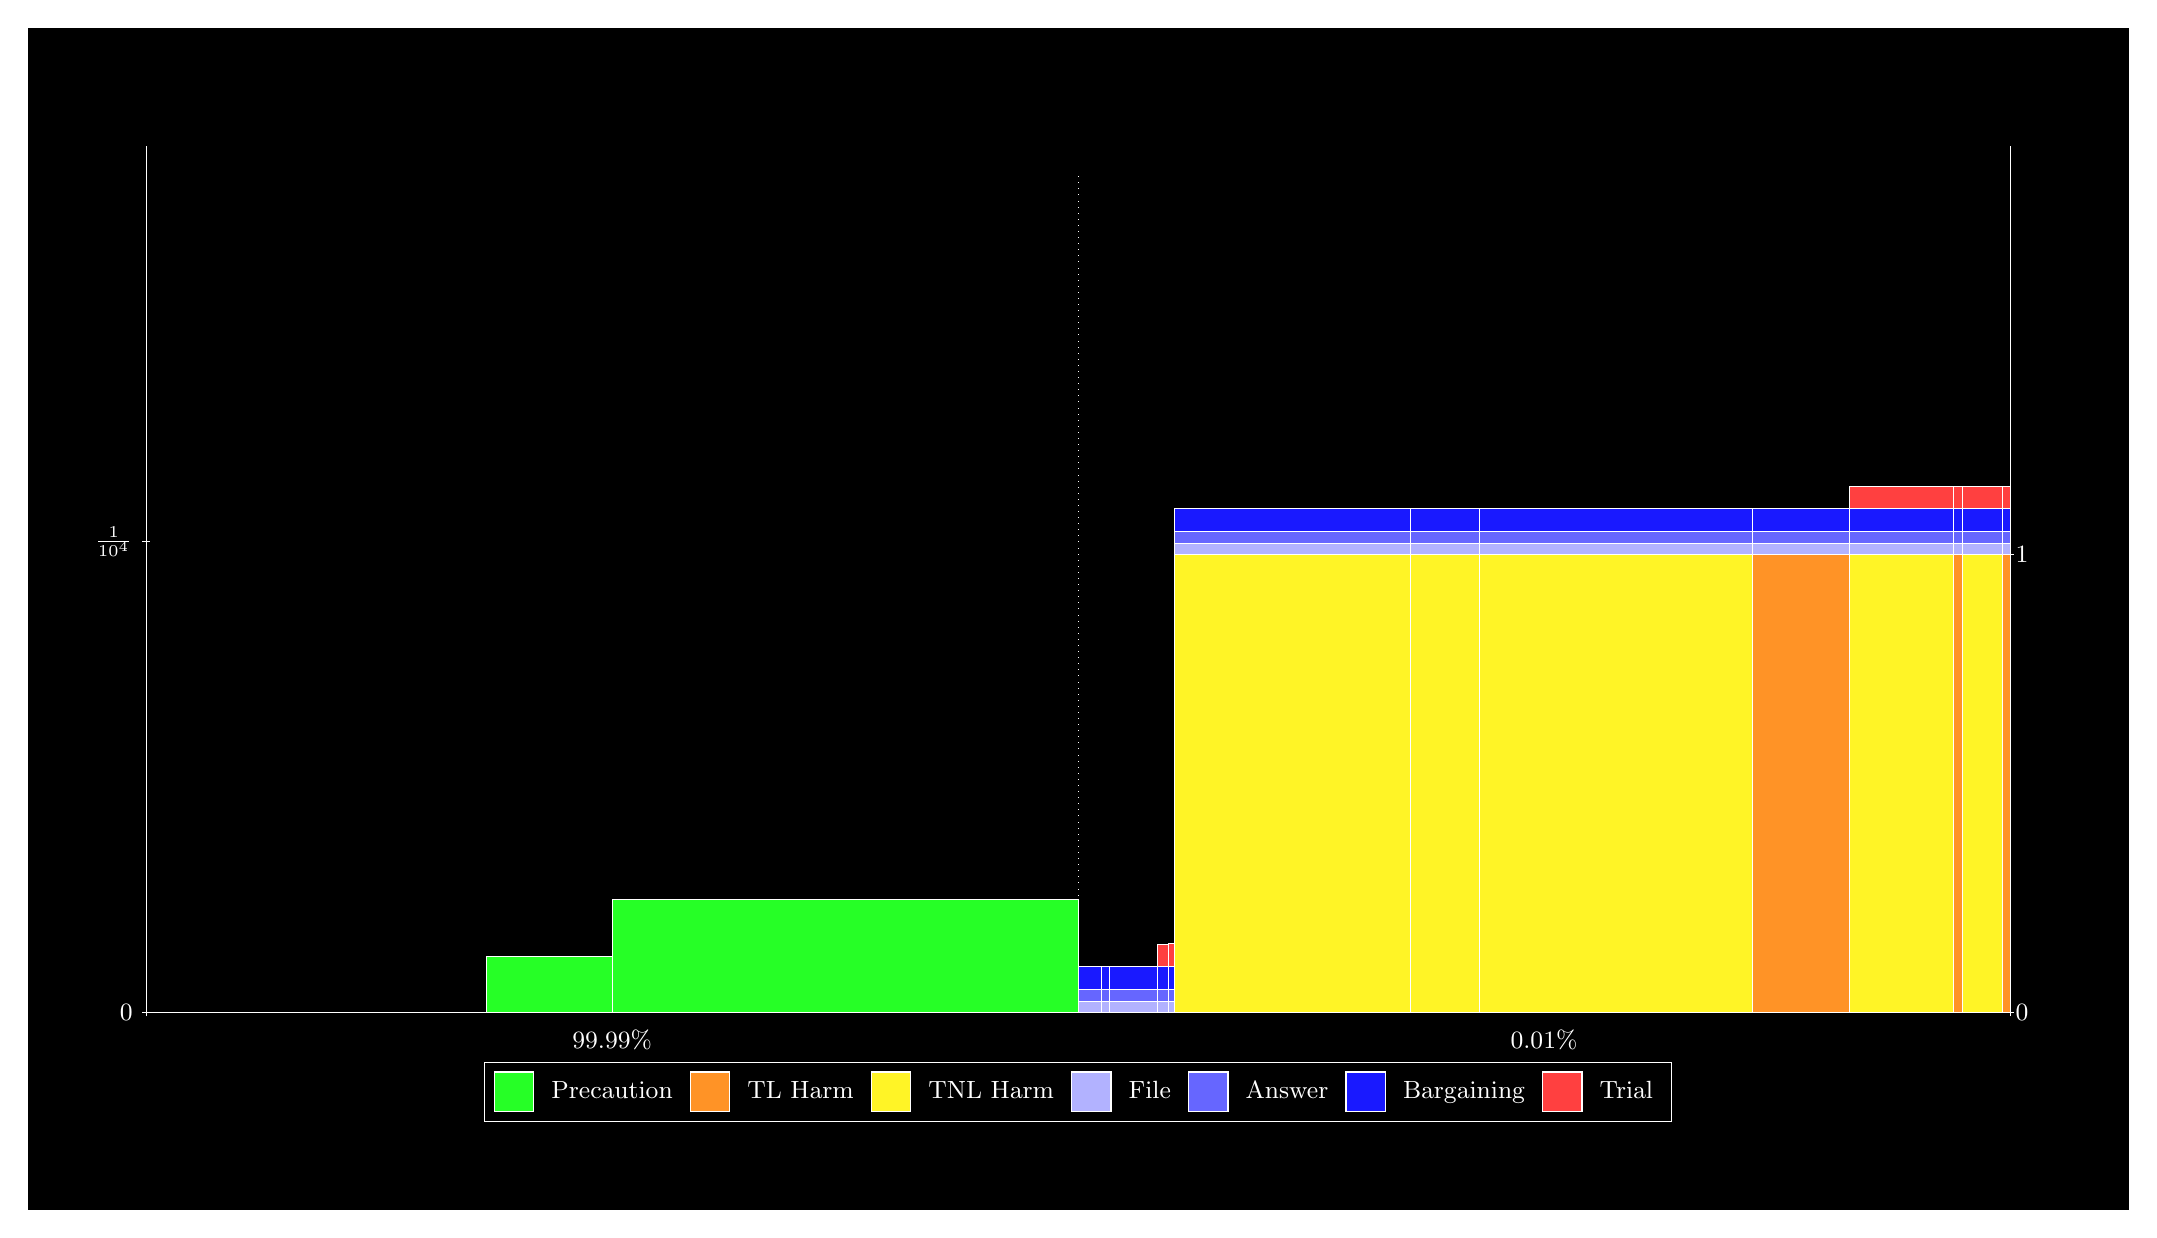
\begin{tikzpicture}
\draw[fill=black] (0,0) rectangle (26.667,15);
\draw[fill=green!85,draw=white,very thin] (5.8206,2.5) rectangle (7.4166,3.2178);
\draw[fill=green!85,draw=white,very thin] (7.4166,2.5) rectangle (13.333,3.9357);
\draw[fill=blue!30,draw=white,very thin] (13.333,2.5) rectangle (13.633,2.6454);
\draw[fill=blue!60,draw=white,very thin] (13.333,2.6454) rectangle (13.633,2.7908);
\draw[fill=blue!90,draw=white,very thin] (13.333,2.7908) rectangle (13.633,3.0816);
\draw[fill=green!85,draw=white,very thin] (13.633,2.5) rectangle (13.73,2.5001);
\draw[fill=blue!30,draw=white,very thin] (13.633,2.5001) rectangle (13.73,2.6455);
\draw[fill=blue!60,draw=white,very thin] (13.633,2.6455) rectangle (13.73,2.7909);
\draw[fill=blue!90,draw=white,very thin] (13.633,2.7909) rectangle (13.73,3.0817);
\draw[fill=green!85,draw=white,very thin] (13.73,2.5) rectangle (14.339,2.5001);
\draw[fill=blue!30,draw=white,very thin] (13.73,2.5001) rectangle (14.339,2.6455);
\draw[fill=blue!60,draw=white,very thin] (13.73,2.6455) rectangle (14.339,2.791);
\draw[fill=blue!90,draw=white,very thin] (13.73,2.791) rectangle (14.339,3.0818);
\draw[fill=blue!30,draw=white,very thin] (14.339,2.5) rectangle (14.483,2.6454);
\draw[fill=blue!60,draw=white,very thin] (14.339,2.6454) rectangle (14.483,2.7908);
\draw[fill=blue!90,draw=white,very thin] (14.339,2.7908) rectangle (14.483,3.0816);
\draw[fill=red!75,draw=white,very thin] (14.339,3.0816) rectangle (14.483,3.3724);
\draw[fill=green!85,draw=white,very thin] (14.483,2.5) rectangle (14.55,2.5001);
\draw[fill=blue!30,draw=white,very thin] (14.483,2.5001) rectangle (14.55,2.6455);
\draw[fill=blue!60,draw=white,very thin] (14.483,2.6455) rectangle (14.55,2.7909);
\draw[fill=blue!90,draw=white,very thin] (14.483,2.7909) rectangle (14.55,3.0817);
\draw[fill=red!75,draw=white,very thin] (14.483,3.0817) rectangle (14.55,3.3725);
\draw[fill=yellow!85,draw=white,very thin] (14.55,2.5) rectangle (17.546,8.3163);
\draw[fill=blue!30,draw=white,very thin] (14.55,8.3163) rectangle (17.546,8.4617);
\draw[fill=blue!60,draw=white,very thin] (14.55,8.4617) rectangle (17.546,8.6071);
\draw[fill=blue!90,draw=white,very thin] (14.55,8.6071) rectangle (17.546,8.8979);
\draw[fill=orange!85,draw=white,very thin] (17.546,2.5) rectangle (17.55,8.3163);
\draw[fill=blue!30,draw=white,very thin] (17.546,8.3163) rectangle (17.55,8.4617);
\draw[fill=blue!60,draw=white,very thin] (17.546,8.4617) rectangle (17.55,8.6071);
\draw[fill=blue!90,draw=white,very thin] (17.546,8.6071) rectangle (17.55,8.8979);
\draw[fill=green!85,draw=white,very thin] (17.55,2.5) rectangle (18.427,2.5001);
\draw[fill=yellow!85,draw=white,very thin] (17.55,2.5001) rectangle (18.427,8.3163);
\draw[fill=blue!30,draw=white,very thin] (17.55,8.3163) rectangle (18.427,8.4617);
\draw[fill=blue!60,draw=white,very thin] (17.55,8.4617) rectangle (18.427,8.6071);
\draw[fill=blue!90,draw=white,very thin] (17.55,8.6071) rectangle (18.427,8.898);
\draw[fill=green!85,draw=white,very thin] (18.427,2.5) rectangle (18.432,2.5001);
\draw[fill=orange!85,draw=white,very thin] (18.427,2.5001) rectangle (18.432,8.3163);
\draw[fill=blue!30,draw=white,very thin] (18.427,8.3163) rectangle (18.432,8.4617);
\draw[fill=blue!60,draw=white,very thin] (18.427,8.4617) rectangle (18.432,8.6071);
\draw[fill=blue!90,draw=white,very thin] (18.427,8.6071) rectangle (18.432,8.898);
\draw[fill=green!85,draw=white,very thin] (18.432,2.5) rectangle (21.894,2.5001);
\draw[fill=yellow!85,draw=white,very thin] (18.432,2.5001) rectangle (21.894,8.3164);
\draw[fill=blue!30,draw=white,very thin] (18.432,8.3164) rectangle (21.894,8.4618);
\draw[fill=blue!60,draw=white,very thin] (18.432,8.4618) rectangle (21.894,8.6072);
\draw[fill=blue!90,draw=white,very thin] (18.432,8.6072) rectangle (21.894,8.898);
\draw[fill=green!85,draw=white,very thin] (21.894,2.5) rectangle (23.122,2.5001);
\draw[fill=orange!85,draw=white,very thin] (21.894,2.5001) rectangle (23.122,8.3164);
\draw[fill=blue!30,draw=white,very thin] (21.894,8.3164) rectangle (23.122,8.4618);
\draw[fill=blue!60,draw=white,very thin] (21.894,8.4618) rectangle (23.122,8.6072);
\draw[fill=blue!90,draw=white,very thin] (21.894,8.6072) rectangle (23.122,8.898);
\draw[fill=yellow!85,draw=white,very thin] (23.122,2.5) rectangle (24.449,8.3163);
\draw[fill=blue!30,draw=white,very thin] (23.122,8.3163) rectangle (24.449,8.4617);
\draw[fill=blue!60,draw=white,very thin] (23.122,8.4617) rectangle (24.449,8.6071);
\draw[fill=blue!90,draw=white,very thin] (23.122,8.6071) rectangle (24.449,8.8979);
\draw[fill=red!75,draw=white,very thin] (23.122,8.8979) rectangle (24.449,9.1887);
\draw[fill=orange!85,draw=white,very thin] (24.449,2.5) rectangle (24.566,8.3163);
\draw[fill=blue!30,draw=white,very thin] (24.449,8.3163) rectangle (24.566,8.4617);
\draw[fill=blue!60,draw=white,very thin] (24.449,8.4617) rectangle (24.566,8.6071);
\draw[fill=blue!90,draw=white,very thin] (24.449,8.6071) rectangle (24.566,8.8979);
\draw[fill=red!75,draw=white,very thin] (24.449,8.8979) rectangle (24.566,9.1887);
\draw[fill=green!85,draw=white,very thin] (24.566,2.5) rectangle (25.069,2.5001);
\draw[fill=yellow!85,draw=white,very thin] (24.566,2.5001) rectangle (25.069,8.3163);
\draw[fill=blue!30,draw=white,very thin] (24.566,8.3163) rectangle (25.069,8.4617);
\draw[fill=blue!60,draw=white,very thin] (24.566,8.4617) rectangle (25.069,8.6071);
\draw[fill=blue!90,draw=white,very thin] (24.566,8.6071) rectangle (25.069,8.898);
\draw[fill=red!75,draw=white,very thin] (24.566,8.898) rectangle (25.069,9.1888);
\draw[fill=green!85,draw=white,very thin] (25.069,2.5) rectangle (25.167,2.5001);
\draw[fill=orange!85,draw=white,very thin] (25.069,2.5001) rectangle (25.167,8.3163);
\draw[fill=blue!30,draw=white,very thin] (25.069,8.3163) rectangle (25.167,8.4617);
\draw[fill=blue!60,draw=white,very thin] (25.069,8.4617) rectangle (25.167,8.6071);
\draw[fill=blue!90,draw=white,very thin] (25.069,8.6071) rectangle (25.167,8.898);
\draw[fill=red!75,draw=white,very thin] (25.069,8.898) rectangle (25.167,9.1888);
\draw[white,very thin] (1.5,2.5) -- (1.5,13.5);
\draw[white,very thin] (1.45,2.5) -- (1.55,2.5);
\node[font=\small,text=white, anchor=east] at (1.45, 2.5) {0};
\draw[white,very thin] (1.45,8.4821) -- (1.55,8.4821);
\node[font=\small,text=white, anchor=east] at (1.45, 8.4821) {$\frac{1}{10^{4}}$};

\draw[white,dotted,very thin] (13.333,2.83) -- (13.333,13.17);
\draw[white,very thin] (25.167,2.5) -- (25.167,13.5);
\draw[white,very thin] (25.117,2.5) -- (25.217,2.5);
\node[font=\small,text=white, anchor=west] at (25.117, 2.5) {0};
\draw[white,very thin] (25.117,8.3163) -- (25.217,8.3163);
\node[font=\small,text=white, anchor=west] at (25.117, 8.3163) {1};

\draw[white,very thin] (1.5,2.5) -- (25.167,2.5);
\draw[white,very thin] (1.5,2.45) -- (1.5,2.55);
\node[font=\small,text=white, anchor=north] at (1.5, 2.45) {};
\draw[white,very thin] (25.167,2.45) -- (25.167,2.55);
\node[font=\small,text=white, anchor=north] at (25.167, 2.45) {};

\node[font=\small,text=white,anchor=south] at (7.4167, 1.9) {99.99\%};
\node[font=\small,text=white,anchor=south] at (19.25, 1.9) {0.01\%};
\draw (13.3333,2.5) node (B) {};
\begin{scope}[align=center]
\matrix[scale=0.5,draw=white,below=0.5cm of B,nodes={draw},column sep=0.1cm]{
\node[rectangle,draw,minimum width=0.5cm,minimum height=0.5cm,fill=green!85]{}; & \node[draw=none,font=\small,text=white]{Precaution}; &
\node[rectangle,draw,minimum width=0.5cm,minimum height=0.5cm,fill=orange!85]{}; & \node[draw=none,font=\small,text=white]{TL Harm}; &
\node[rectangle,draw,minimum width=0.5cm,minimum height=0.5cm,fill=yellow!85]{}; & \node[draw=none,font=\small,text=white]{TNL Harm}; &
\node[rectangle,draw,minimum width=0.5cm,minimum height=0.5cm,fill=blue!30]{}; & \node[draw=none,font=\small,text=white]{File}; &
\node[rectangle,draw,minimum width=0.5cm,minimum height=0.5cm,fill=blue!60]{}; & \node[draw=none,font=\small,text=white]{Answer}; &
\node[rectangle,draw,minimum width=0.5cm,minimum height=0.5cm,fill=blue!90]{}; & \node[draw=none,font=\small,text=white]{Bargaining}; &
\node[rectangle,draw,minimum width=0.5cm,minimum height=0.5cm,fill=red!75]{}; & \node[draw=none,font=\small,text=white]{Trial}; \\\\
};\end{scope}

\end{tikzpicture}
\end{document}